% ------------------------------------------------------------
% ACM sig-alternate submission block samples created by yuanchao shu @ 2015
% ------------------------------------------------------------

%!TEX root = main.tex

\newpage

\section{Examples}
\label{sec:sample}

\subsection{subsection}
\label{subsec:2.1}
\subsection{subsubsection}
\label{subsubsec:2.1.1}

Cite \autoref{sec:sample}, \autoref{subsec:2.1}, \autoref{subsubsec:2.1.1}

\begin{lemma}\label{lm:1}
This is a lemma.
\end{lemma}
Cite \autoref{lm:1}

\begin{corollary}\label{cl:1}
This is a corollary.
\end{corollary}
Cite \autoref{cl:1}

\begin{theorem}\label{th:1}
This is a theorem.
\end{theorem}
Cite \autoref{th:1}

\begin{figure}[!htb]
%\vspace{-12pt}
  \begin{center}
      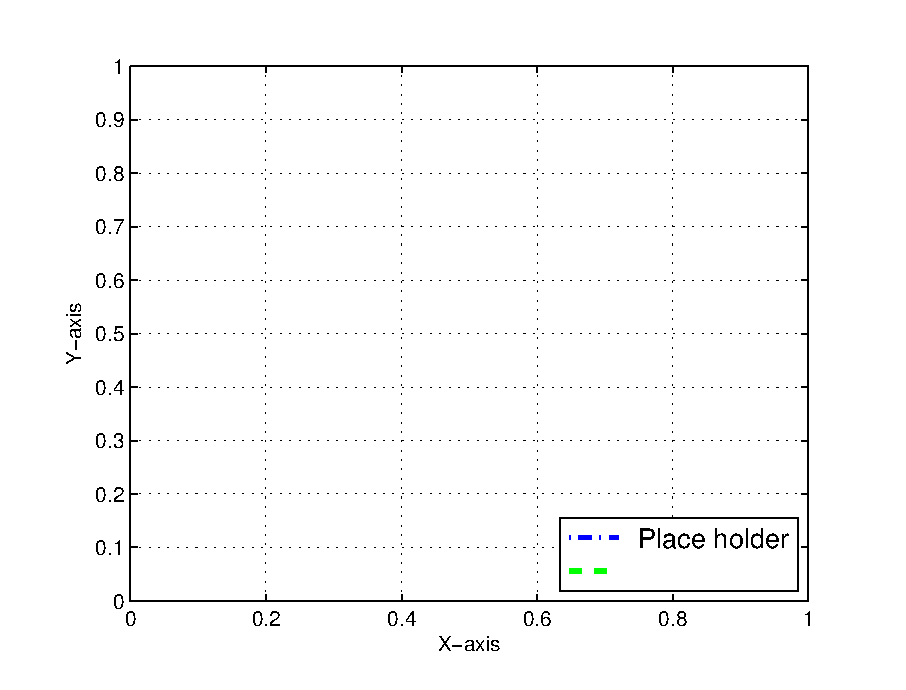
\includegraphics[width=0.4\textwidth]{placeholder}
      % \vspace{-3pt}
      \caption{A placeholder.}\label{fig:placeholder0}
  \end{center}
% \vspace{-12pt}
\end{figure}

\begin{figure}[!htb]
%\vspace{-12pt}
  \begin{center}
      \subfigure[placeholder.]{
      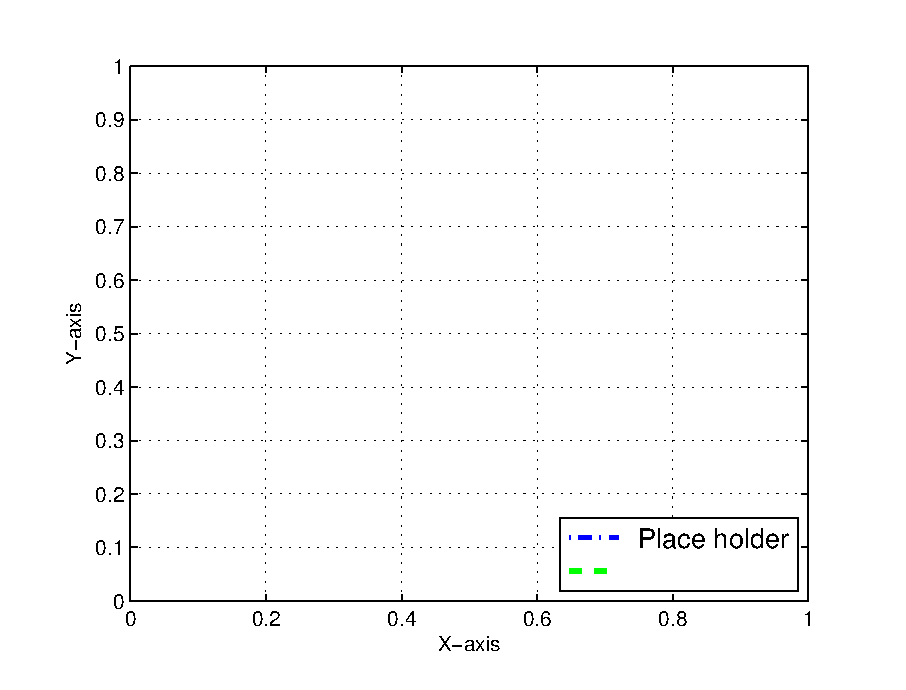
\includegraphics[width=0.21\textwidth]{placeholder}
      \label{fig:placeholder11}}
      %\hspace{-8pt}
      \subfigure[placeholder.]{
      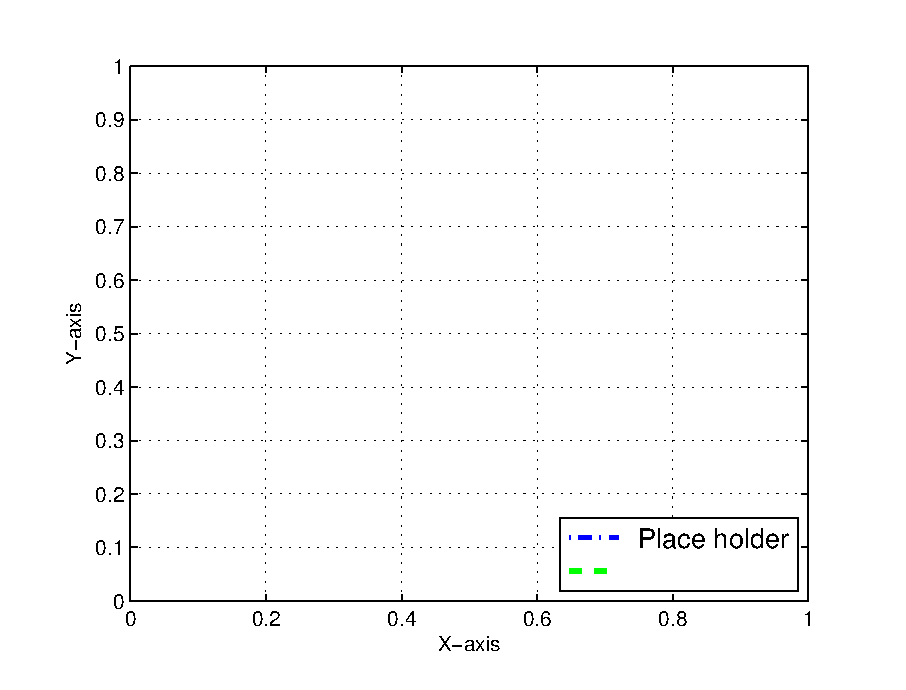
\includegraphics[width=0.21\textwidth]{placeholder}
      \label{fig:placeholder12}}
      % \vspace{-3pt}
      \caption{A placeholder.}\label{fig:placeholder1}
  \end{center}
% \vspace{-15pt}
\end{figure}

\begin{figure*}[!htb]
%\vspace{-12pt}
  \begin{center}
      \subfigure[placeholder.]{
      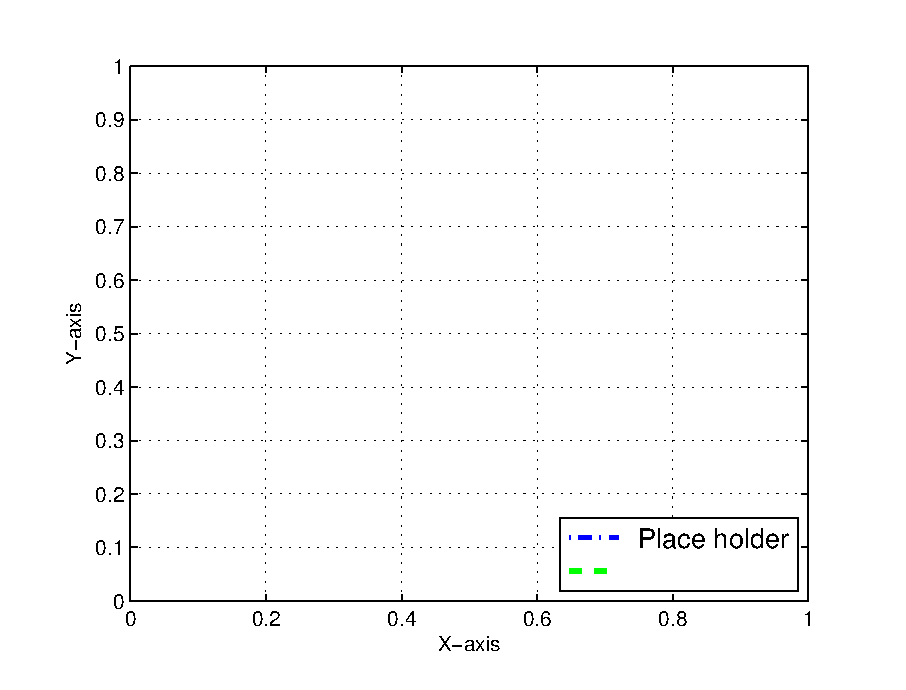
\includegraphics[width=0.31\textwidth]{placeholder}
      \label{fig:placeholder21}}
      %\hspace{-8pt}
      \subfigure[placeholder.]{
      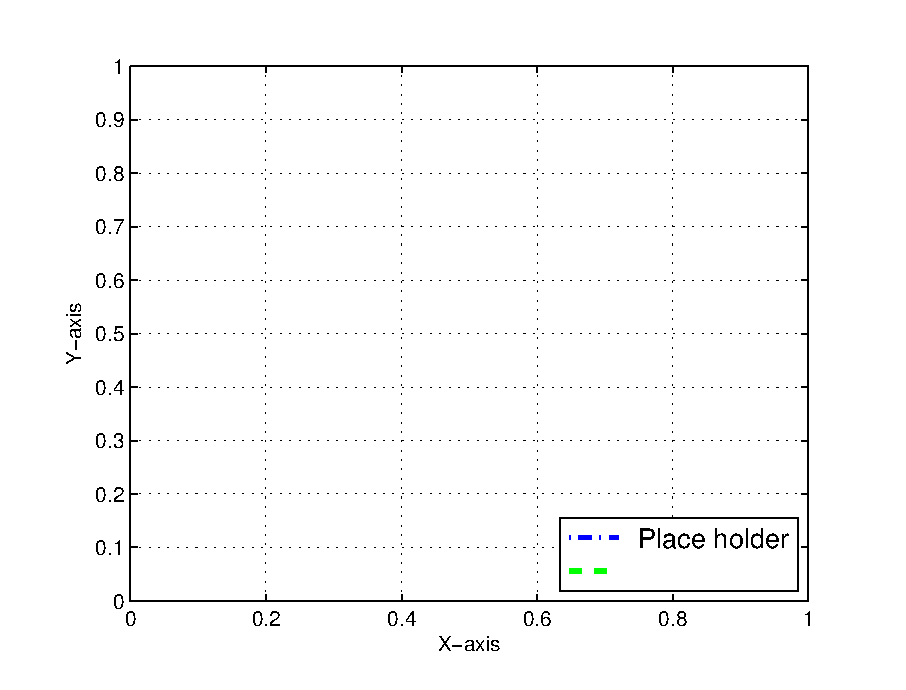
\includegraphics[width=0.31\textwidth]{placeholder}
      \label{fig:placeholder22}}
      % \vspace{-3pt}
      \subfigure[placeholder.]{
      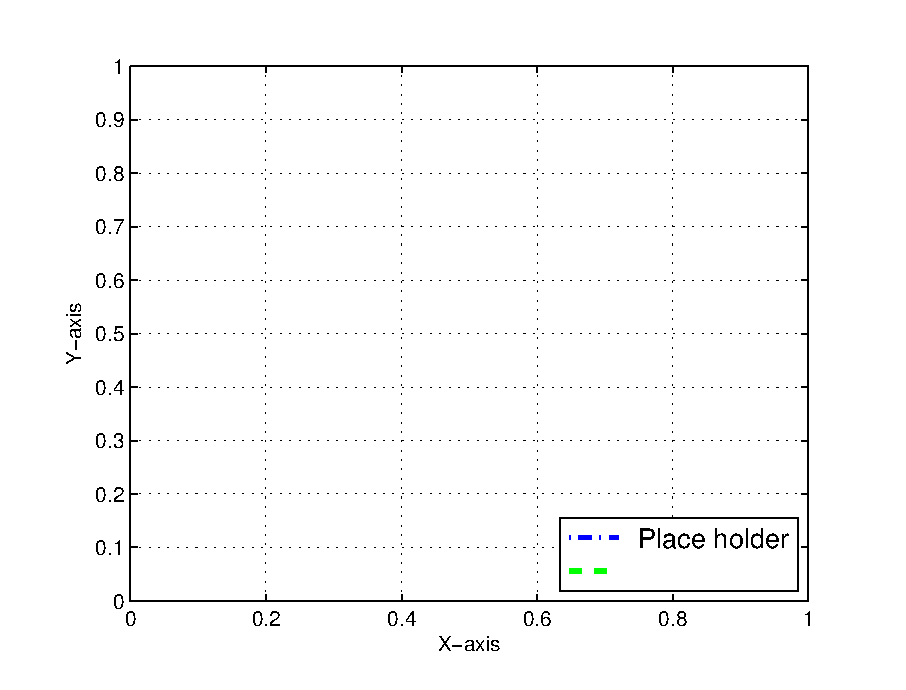
\includegraphics[width=0.31\textwidth]{placeholder}
      \label{fig:placeholder23}}
      % \vspace{-3pt}
      \caption{A placeholder.}\label{fig:placeholder2}
  \end{center}
% \vspace{-15pt}
\end{figure*}

\begin{figure*}[!htb]
    \begin{minipage}[t]{0.33\linewidth}
        \centering
        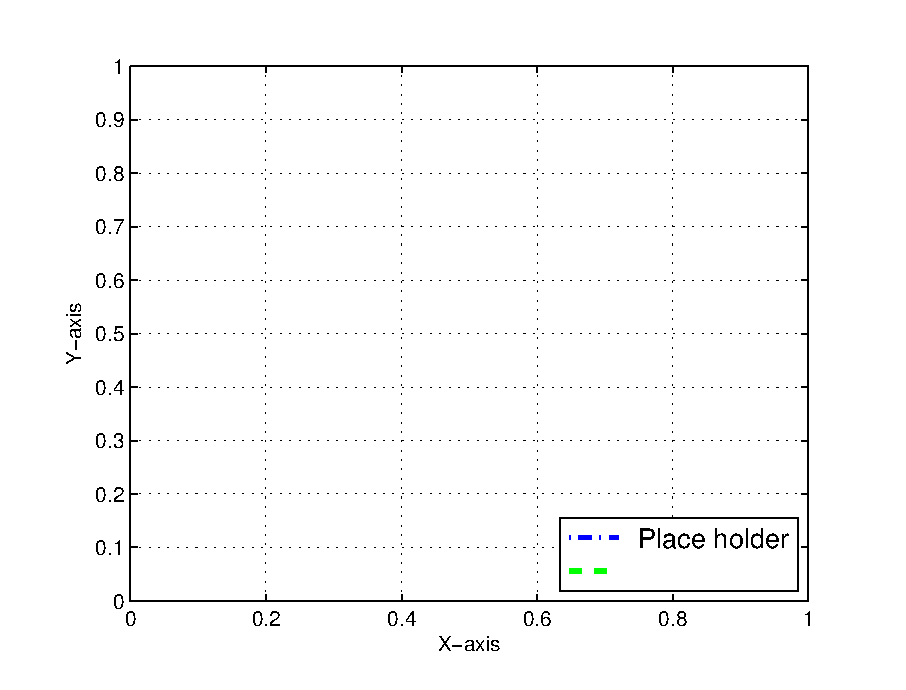
\includegraphics[width=5.8cm]{placeholder}
        \caption{placeholder.}
        \label{fig:placeholder31}
    \end{minipage}
    \hfill
    \begin{minipage}[t]{0.33\linewidth}
        \centering
        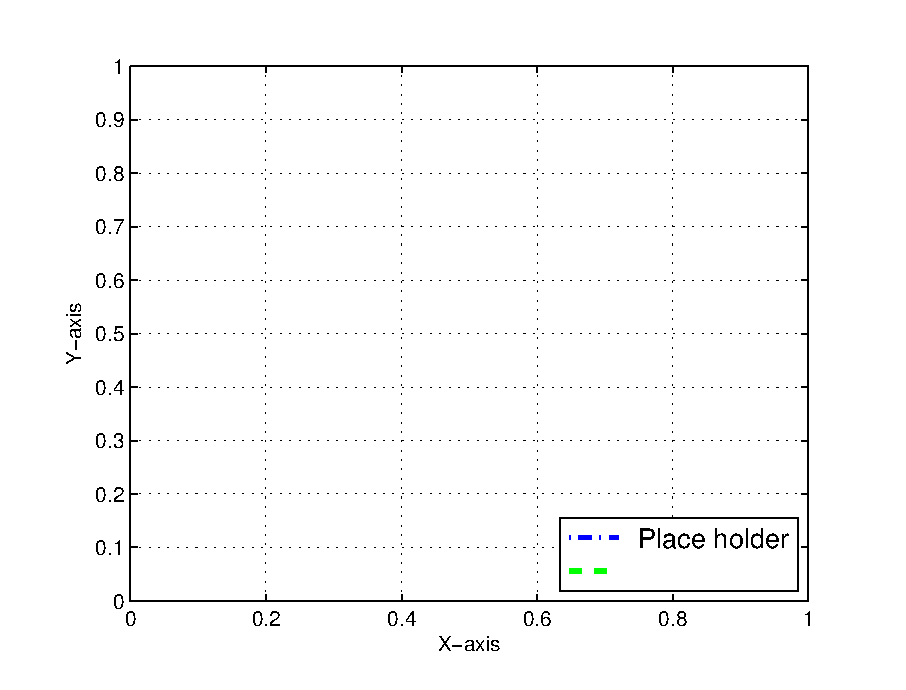
\includegraphics[width=5.8cm]{placeholder}
        \caption{placeholder.}
        \label{fig:placeholder32}
    \end{minipage}
    \hfill
    \begin{minipage}[t]{0.33\linewidth}
        \centering
        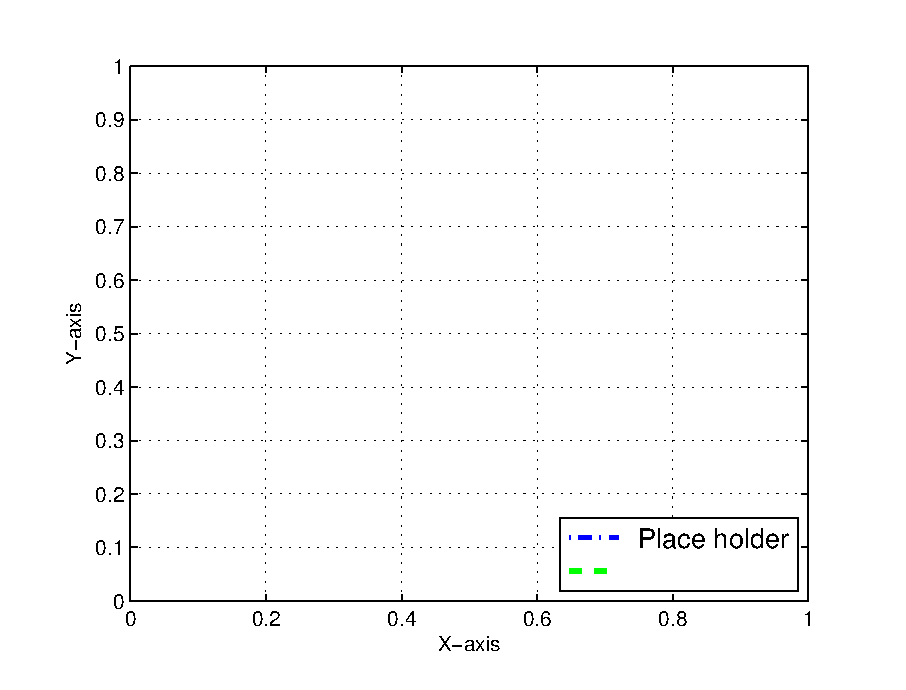
\includegraphics[width=5.8cm]{placeholder}
        \caption{placeholder.}
        \label{fig:placeholder33}
    \end{minipage}
    %\vspace{-0.05in}
\end{figure*}
Cite \autoref{fig:placeholder0}, \autoref{fig:placeholder1}, \autoref{fig:placeholder11}, \autoref{fig:placeholder12}, \autoref{fig:placeholder2}, \autoref{fig:placeholder21}, \autoref{fig:placeholder22}, \autoref{fig:placeholder23}, \autoref{fig:placeholder31}, \autoref{fig:placeholder32}, \autoref{fig:placeholder33}

\begin{algorithm}[!htb]
\SetKwInOut{Input}{Input}\SetKwInOut{Output}{Output}
\SetKwFunction{MagPreprocess}{MagPreprocess}
\SetKwProg{Fn}{Function}{}{end}
\Input{$v = \{t^v, m^v, s^v, tr^v, l^v\}$}
\Output{$uv$ where $uv_i = j$}
%\Begin{
$p_u = 0$, $p_v = 0$, $p_u^{inc} = true$\;
\For{each sample $m^v_i \in m^v$}{
    $m^{vp}_i$ = f($m^v_i$)\;
}
\While{$p_v \leq size(v)$}{
    \If{$p_u^{inc}$}{
        $uv_i = \arg\min D[k][p_u]$, $k \in [p_v - c, p_v]$\;
        \For{each observation $u_i$}{
            get $a^u_i$, $m^u_i$\;
            $m^{up}_i$ = f($m^u_i$)\;
        }
    }
}
\caption{algorithm example}\label{alg:1}
\end{algorithm}
Cite \autoref{alg:1}

\begin{table}[!htb]%\footnotesize
  \caption{table example}\label{table:1}
  \begin{center}
    \begin{tabular}{|c|c|}
   % \begin{tabular*}{84mm}{|c|c|}
      \hline
      \hline
      aaaa & $m = <t_i, m^x_i, m^y_i, m^z_i>$ \\
      \hline
      bbbb & $s = <t_i, s_i>$, $s_i = 1, 2, 3,\ldots$ \\
      \hline
      \hline
    \end{tabular}
  \end{center}
% \vspace{-12pt}
\end{table}
Cite \autoref{table:1}

Cite \cite{john00}